\section{Experiments}
\label{sec:experiments}
\subsection{Setup and Scope}
\paragraph{Data and adaptation.}
The 419-hour policy-pretraining corpus combines HIW-500, 14 G1 task subsets from UniFoLM-WBT, and Humanoid Everyday~\cite{humanoid_everyday}. We use only the dataset snapshot available when the corpus was assembled. Policy pretraining runs for one million steps with batch size 1024 on 16 H200 GPUs. Target-task training uses the same frozen motion backbone for both initialization variants. The policy has 678M total and approximately 92M trainable parameters; supplementary material reports the optimization settings.

\paragraph{Evaluation.}
HumanoidArena~\cite{humanoidarena} contains seven tasks, with 100 demonstrations per task. We test separate single-task policies and one jointly trained policy, reporting success rate (SR) and average fall rate (AFR). SIMPLE~\cite{simple} is evaluated on eight released tasks under L0--L2 visual, lighting, and target-pose variation. Each table entry aggregates 30 trials, ten per level. Physical experiments use a G1 with a D435i camera and Dex3-1 hands, 25--30 demonstrations per task, and ten trials on each of eight tasks.

We distinguish results in our original benchmark comparison from literature-reported rows added to the comparison tables. HuGe results come from its Table~4~\cite{liu2026huge}; additional HumanoidArena baselines come from Table~1 of Language-Forcing~\cite{li2026languageforcing}. Several SIMPLE task results come from Memory before Goal~\cite{chen2026memorybeforegoal}. These rows broaden context but are not controlled re-runs with a common pretraining corpus and evaluation implementation. Missing results are not treated as zero. We report descriptive comparisons and do not infer statistical significance from small aggregate differences.

\subsection{Simulation Results}
\paragraph{Multi-task HumanoidArena.}
Table~\ref{tab:arena_summary} summarizes all comparison rows; per-task values and available deviations are in the supplement. \ours$^{*}$ achieves 72.14\% overall SR, 2.44 percentage points above the highest listed baseline aggregate (GR00T N1.7, 69.70\%). Against the original $\pi_{0.5}$ comparison (53.8\%), the difference is about 18.3 points. The policy has the highest HSI mean (84.17\%) and lowest reported AFR (4.29\%), while its HOI mean (56.11\%) is lower than GR00T N1.7 (62.22\%). Thus its aggregate advantage does not imply uniformly stronger object interaction.

Additional policy pretraining improves our multi-task mean from 67.63\% to 72.14\%. It improves P\&Pbox, OpenDoor, Boxing, and VisNavi, matches SitSofa, and changes Football and DoubleDesk in opposite directions. The strongest task results include P\&Pbox (90.0\%), OpenDoor (95.0\%), SitSofa (96.7\%), and VisNavi (76.7\%). RTC is disabled for both variants.

\begin{table}[t]
\centering\small
\caption{\textbf{Multi-task HumanoidArena.} Baselines include ACT~\cite{ACT}, DP~\cite{chi2023diffusionpolicy}, FM~\cite{FM_objective}, and $\pi_{0.5}$~\cite{pi05}. All values are percentages. HOI/HSI denote object/scene interaction means; lower AFR is better. $\ddagger$: HuGe Table~4~\cite{liu2026huge}; $\dagger$: Language-Forcing Table~1~\cite{li2026languageforcing}. Literature rows have no reported AFR here. $^{*}$ denotes our additional policy pretraining.}
\label{tab:arena_summary}
\setlength{\tabcolsep}{3.3pt}
\begin{tabular}{lrrrr}\toprule
Method & HOI & HSI & Overall & AFR\\\midrule
ACT &36.7&41.7&39.5&7.4\\
DP &29.4&59.6&46.7&7.1\\
FM &13.9&45.4&31.9&7.1\\
$\pi_{0.5}$ &38.3&65.4&53.8&6.4\\
HuGe-OFT$^{\ddagger}$ &33.89&69.17&54.05&--\\
HuGe-GR00T$^{\ddagger}$ &56.11&74.58&66.67&--\\
HuGe-Pi$^{\ddagger}$ &50.56&75.83&65.00&--\\
Fast-WAM$^{\dagger}$ &55.00&65.73&61.13&--\\
LingBot-VA$^{\dagger}$ &56.95&71.67&65.36&--\\
GR00T N1.7$^{\dagger}$ &\textbf{62.22}&75.31&69.70&--\\
GigaWorld$^{\dagger}$ &60.14&74.58&68.39&--\\\midrule
Ours &51.67&79.6&67.63&5.00\\
Ours$^{*}$ &56.11&\textbf{84.17}&\textbf{72.14}&\textbf{4.29}\\\bottomrule
\end{tabular}
\end{table}


\paragraph{Single-task HumanoidArena.}
With a separate policy for each task, direct target-task adaptation reaches 69.51\% overall SR, versus 60.0\% for DP~\cite{chi2023diffusionpolicy}, and 4.29\% AFR. Additional policy pretraining reaches 67.14\%, despite improving OpenDoor and VisNavi. The 2.37-point lower average shows that robot policy pretraining is not uniformly beneficial under the single-task adaptation schedule. Direct adaptation changes from 69.51\% in the single-task setting to 67.63\% in the joint setting, a 1.88-point reduction. Full single-task results are retained in the supplementary material.

\paragraph{SIMPLE.}
Table~\ref{tab:simple_summary} reports aggregate per-task SRs; the supplement preserves the L0/L1/L2 trial counts and all baselines. \ours$^{*}$ reaches 75.83\% over 240 task-level trials, versus 75.42\% for $\Psi_0$, a difference of one successful trial. We therefore describe these policies as competitive overall. Our policy leads on Handover, Mobile P\&P, and OpenFaucet, and ties the best result on CloseDoor and Push Office Chair. It is below $\Psi_0$ on XMoveBendPick and OpenTrashCan, and below InternVLA-M1 on OpenOven (56.7\% versus 73.3\%). These task-dependent outcomes temper claims of broad superiority under perturbation.

\begin{table}[t]
\centering\small
\caption{\textbf{SIMPLE success rates (\%).} Each cell aggregates 30 trials across L0--L2. ACT and InternVLA-M1 (IV-M1) results for the last five tasks are from~\cite{chen2026memorybeforegoal}. Full results include methods with partial task coverage; no eight-task average is assigned to those methods.}
\label{tab:simple_summary}
\setlength{\tabcolsep}{3.0pt}
\begin{tabular}{lrrrr}\toprule
Task & ACT & IV-M1 & $\Psi_0$ & Ours$^{*}$\\\midrule
Handover &46.7&0.0&80.0&\textbf{83.3}\\
Mobile P\&P &60.0&0.0&60.0&\textbf{70.0}\\
XMoveBendPick &73.3&50.0&\textbf{93.3}&80.0\\
CloseDoor &\textbf{100.0}&0.0&\textbf{100.0}&\textbf{100.0}\\
OpenOven &6.7&\textbf{73.3}&53.3&56.7\\
OpenFaucet &3.3&0.0&33.3&\textbf{53.3}\\
Push Office Chair &96.7&20.0&\textbf{100.0}&\textbf{100.0}\\
OpenTrashCan &50.0&0.0&\textbf{83.3}&63.3\\\midrule
Eight-task mean &54.58&17.92&75.42&\textbf{75.83}\\\bottomrule
\end{tabular}
\end{table}


\subsection{Physical-Robot Evaluation}
Figure~\ref{fig:real} shows representative executions. Table~\ref{tab:real} gives per-task successful trial counts. Direct adaptation achieves 36/80 successes (45\%), compared with 25/80 for GR00T N1.6 and 28/80 for $\Psi_0$. Policy-pretrained initialization reaches 48/80 (60\%), improving seven tasks and matching Cart Pushing. The largest absolute success rates are Punching Bag (90\%), Cushion Sitting (80\%), and Dual-Arm PNP (70\%). These are small-sample deployment results on the evaluated tasks, not estimates of unrestricted real-world generalization. RTC is used for our real-world execution; its contribution is not isolated by these comparisons.

\begin{figure*}[t]
\centering
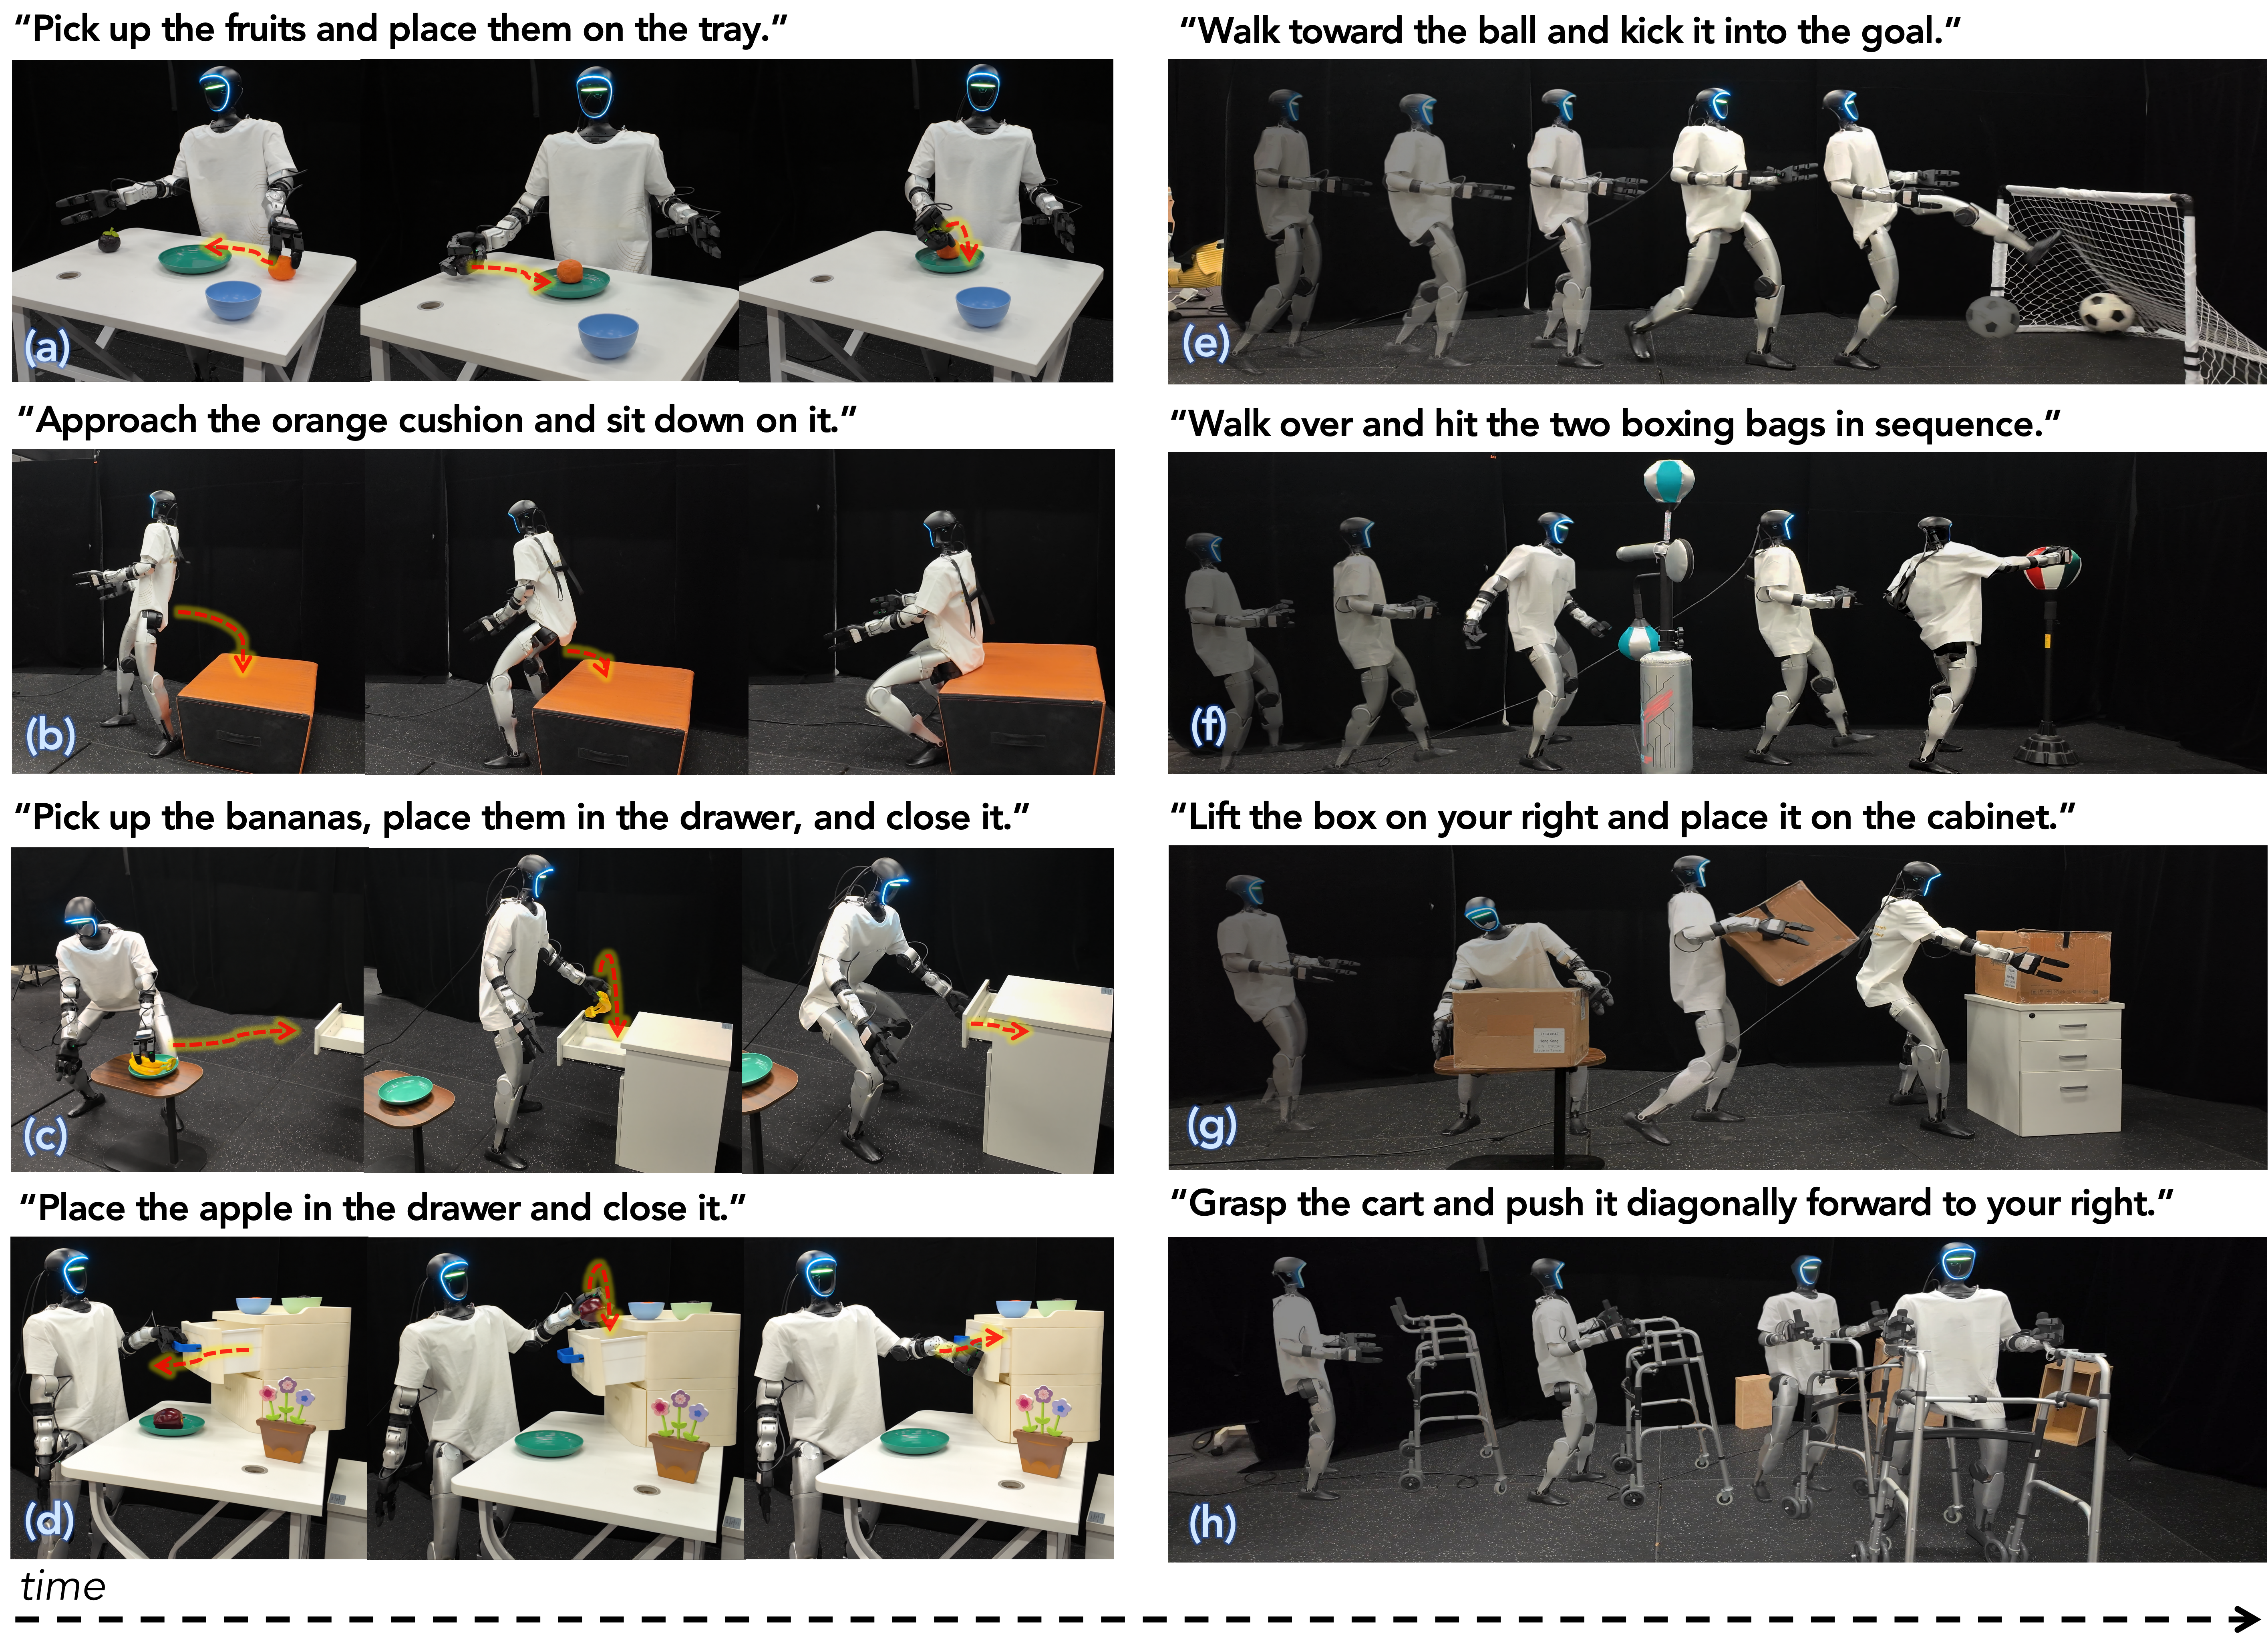
\includegraphics[width=0.82\textwidth]{image/real_world.png}
\caption{\textbf{Physical execution across diverse interactions.} Representative sequences from the eight-task evaluation include object transfer, kicking, sitting, pushing, and carrying. Evaluation uses ten trials per task; quantitative results are in Table~\ref{tab:real}.}
\label{fig:real}
\end{figure*}
\begin{table}[t]
\centering\small
\caption{\textbf{Physical-robot successes / 10 trials.} GR00T denotes N1.6. Ours and Ours$^{*}$ both use a pretrained motion backbone; $^{*}$ adds robot policy pretraining.}
\label{tab:real}
\setlength{\tabcolsep}{3.0pt}
\begin{tabular}{lrrrr}\toprule
Task & GR00T & $\Psi_0$ & Ours & Ours$^{*}$\\\midrule
Single-Arm PNP &2&1&3&4\\
Dual-Arm PNP &4&7&5&7\\
Football Scoring &2&0&2&5\\
Banana Cabinet &3&1&2&4\\
Cart Pushing &3&5&6&6\\
Punching Bag &5&6&8&9\\
Box Carrying &2&3&3&5\\
Cushion Sitting &4&5&7&8\\\midrule
Total / 80 &25&28&36&48\\
Mean (\%) &31.25&35.00&45.00&60.00\\\bottomrule
\end{tabular}
\end{table}


\subsection{What Transfers from the Motion Backbone?}
\paragraph{Motion-prior and adaptation ablations.}
Table~\ref{tab:ablation} reports mean success on DoubleDesk, Football, and P\&Pbox after training on the joint seven-task suite. Without additional policy pretraining, the reference model reaches 51.67\%. Removing the pretrained T2M backbone reduces success to 18.33\%; unfreezing it yields 31.67\%. Replacing MSE with the original Kimodo motion objective yields 35.00\%, and removing root--body gradient detachment yields 45.00\%. These comparisons support retaining the pretrained generator and using direct target supervision with controlled cross-stage gradient flow. They do not separately establish the contribution of each visual-fusion path or of the hand architecture, for which we have no isolated ablation.

Additional policy pretraining increases the three-task mean to 56.11\%. This complements the motion prior rather than replacing it: both compared models retain the same pretrained backbone. The largest change in this analysis is associated with removing motion pretraining, while the gain from additional robot supervision is smaller.
\begin{table}[t]
\centering\small
\caption{\textbf{Three-task ablation.} Mean SR on DoubleDesk, Football, and P\&Pbox after joint seven-task training. Except for the final row, no additional robot policy pretraining is used.}
\label{tab:ablation}
\begin{tabular}{lr}\toprule
Configuration & SR (\%)\\\midrule
Reference (frozen T2M, MSE, detach) &51.67\\
Without pretrained T2M &18.33\\
Unfreeze motion backbone &31.67\\
Original Kimodo motion objective &35.00\\
Without root--body detach &45.00\\
Reference + policy pretraining &56.11\\\bottomrule
\end{tabular}
\end{table}


\paragraph{Matched-capacity backbone comparison.}
With the policy architecture and adaptation protocol fixed, Kimodo-G1-SEED-v1 and RP-v1 (both 282M parameters) yield 64.29\% and 67.63\% overall HumanoidArena success. Their motion corpora contain 288 and 700 hours, including the train/test splits. RP-v1 improves DoubleDesk, P\&Pbox, OpenDoor, and SitSofa, but reduces Football, Boxing, and VisNavi. The 3.34-point aggregate gain is therefore task dependent. Since corpus identity and size change together, this comparison demonstrates sensitivity to the pretrained backbone, rather than isolating data quantity or proving that every measure of text-to-motion quality predicts control performance.

\paragraph{Data and capacity trends.}
Across three policy-pretraining data scales (105/210/419 hours), multi-task success is 68.10/69.05/72.14\%. In a separate capacity sweep (53.6/91.7/158.9M active parameters), success is 61.43/67.63/68.57\%. These monotonic observations support further scaling studies within the evaluated setup, but three points do not establish a scaling law. The data and capacity sweeps are separate experiments and their endpoints should not be conflated. Full backbone results and the scaling curves are provided in the supplement.
